\subsection{Surface Enhanced Raman Spectroscopy with Graphene}

\begin{figure}[!h]
  \centering
  \begin{subfigure}{0.45\textwidth}
    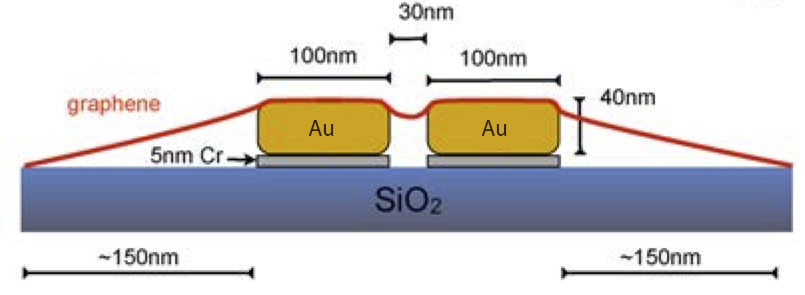
\includegraphics[width=\textwidth]{./images/sers-schema.png}
  \end{subfigure}
  ~
  \begin{subfigure}{0.45\textwidth}
    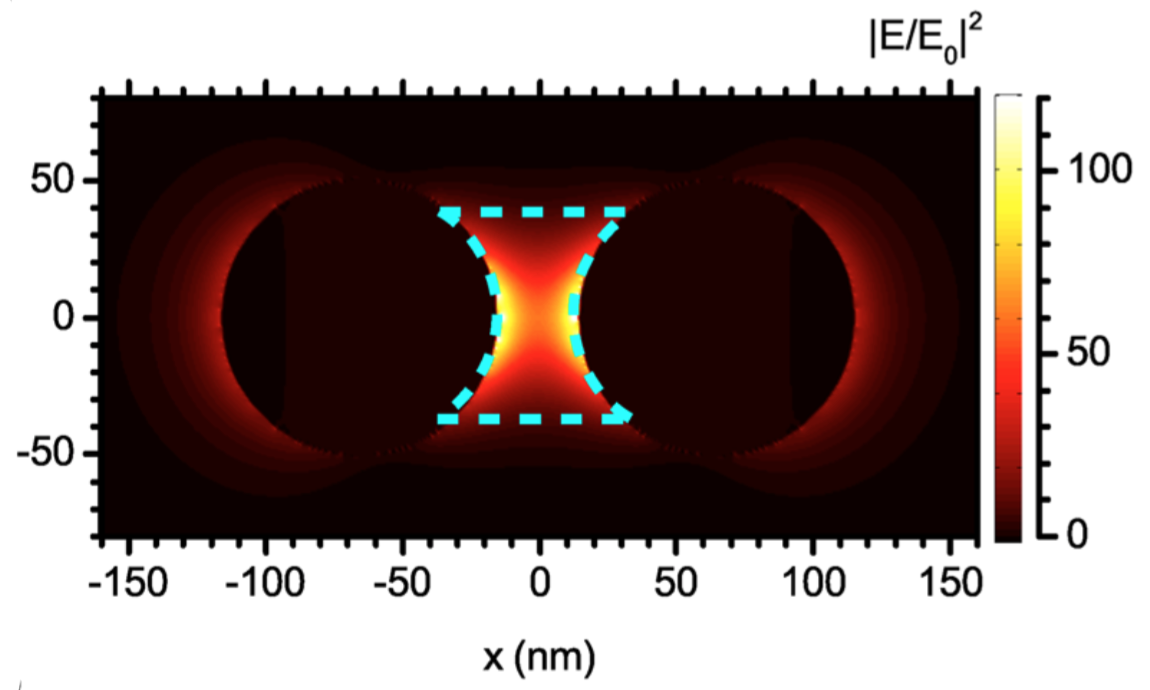
\includegraphics[width=\textwidth]{./images/local-enhancement-heeg.png}
  \end{subfigure}
  \caption{\textbf{(a)} Gold disks are placed with a chrome interlayer on SiO$_2$. A layer of graphene is pulled into the gap. Adapted from \cite{heeg}. \textbf{(b)} Local enhancement at $\lambda = 638nm$ and $z=40nm$. The blue dashed line indicates the area that includes 90\% of the near field intensity according to \cite{heeg}. Copied from \cite{heeg}.}
\end{figure}

\note{komponente des E-felds parallel zum raman dipolmoment erzeugt verstärkung, für graphen: nur Komponente des Nahfelds in der Graphen Ebene zählt}
